

The preselection sample is based on the following criteria
\begin{itemize}
\item satisfy the trigger requirement (see
  Table.~\ref{tab:DatasetsData})
\item select events with one high \pt\ electron or muon, requiring
  \begin{itemize}
  \item $\pt>30~\GeVc$ and $|\eta|<2.5(2.1)$ for \E(\M)
  \item satisfy the identification and isolation requirements detailed
    in~\cite{ref:osznote} for electrons and in~\cite{ref:osznote} for muons
  \end{itemize} 
  \item require at least 4 PF jets in the event with $\pt>30~\GeV$
    within $|\eta|<2.5$, out of which at least 1 is b-tagged based on
    the SSV medium working point [CITE]. 
  \item require moderate $\met>50~\GeV$
\end{itemize}

A benchmark signal sample is selected by tightening the \met\ and
adding an \mt\ requirement
\begin{itemize}
\item $\met>100~\GeV$
\item $\mt>150~\GeV$
\end{itemize}

\subsection{Corrections to Jets and \met}

The official recommendations from the Jet/MET group are used for 
the data and MC samples. In particular, the jet
energy corrections (JEC) are updated using the official recipe.
L1FastL2L3Residual (L1FastL2L3) corrections are applied for data (MC),
based on the global tags GR\_R\_42\_V23 (DESIGN42\_V17) for
data (MC). In addition, these jet energy corrections are propagated to
the \met\ calculation, following the official prescription for
deriving the Type I corrections. It may be noted that events with
anomalous corrections are excluded from the sample since these 
correspond to events with unphysically large \met\ and \mt\ tail
signal region. An additional correction to remove
the $\phi$-modulation observed in the \met\ is included, improving 
the agreement between the data and the MC, as shown in 
Figure.~\ref{fig:metphicomp}. This correction has an effect on this analysis,
since the azimuthal angle enters the \mt\ distribution. 

\begin{figure}[tbh]
  \begin{center}
	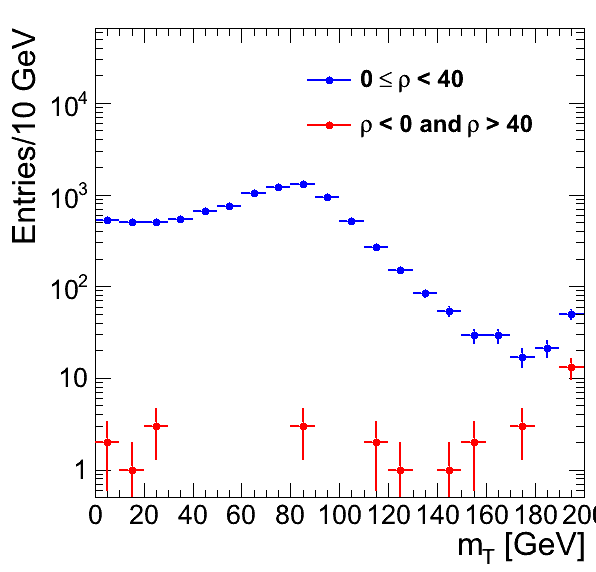
\includegraphics[width=0.5\linewidth]{plots/mt_rho_comp.png}
	\caption{ \label{fig:mtrhocomp}%\protect 
	  Comparison of the \mt\ distribution for events with
          unphysical energy corrections ($\rho <0$ or $ \rho > 40$, where $\rho$ is a
          measure of the average pileup energy density) and the
          nominal sample. Events with large pileup corrections 
          correspond to noisy events. Since this correction is applied
          to the jets and propagated to the \met, these events have
          anomalously large \met\ and populate the \mt\ tail. These
          pathological events are excluded from the analysis sample.}
  \end{center}
\end{figure}

\begin{figure}[hb]
  \begin{center}
	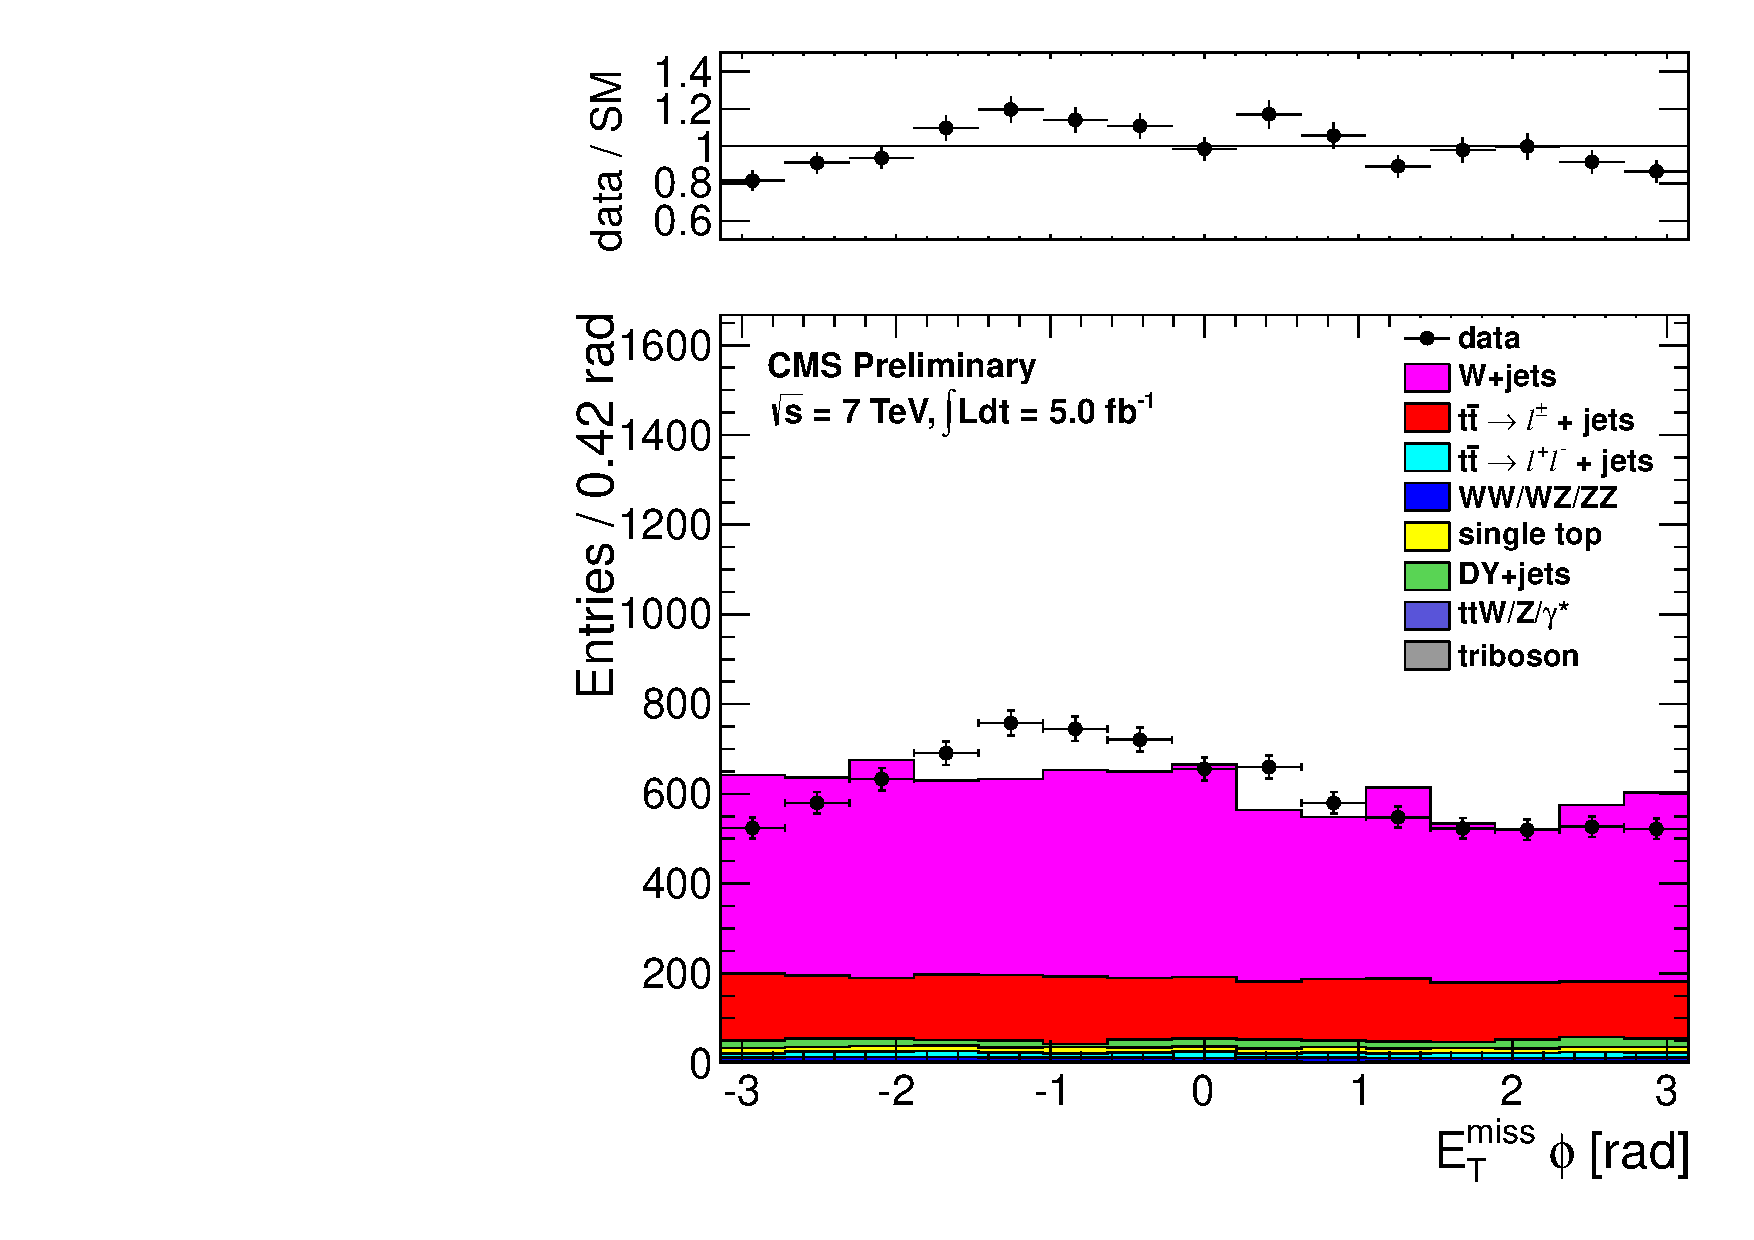
\includegraphics[width=0.5\linewidth]{plots/metphi.pdf}%
	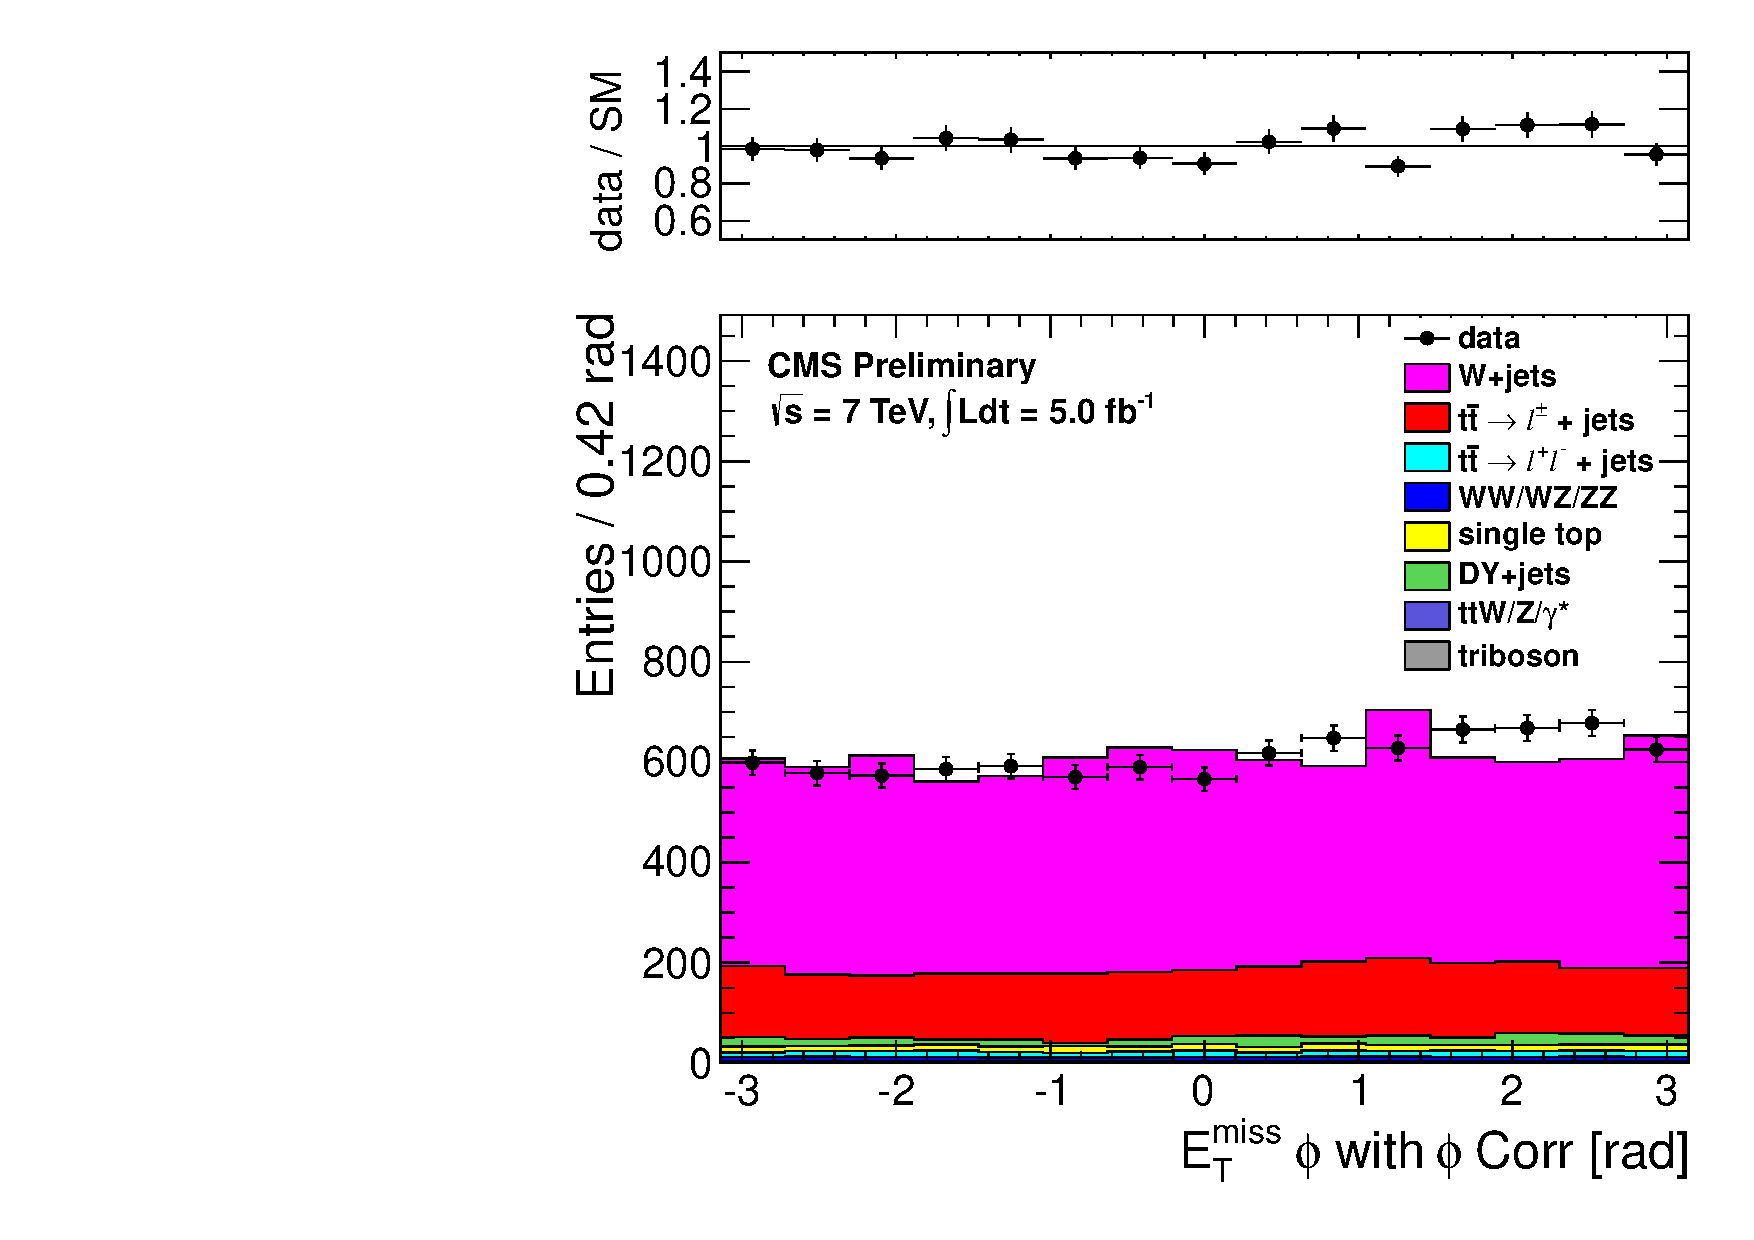
\includegraphics[width=0.5\linewidth]{plots/metphi_phicorr.pdf}
	\caption{ \label{fig:metphicomp}%\protect 
	  The PF \met\ $\phi$ distribution (left) exhibits a
          modulation. After applying a dedicated correction, the
          azimuthal dependence is reduced (right).}
  \end{center}
\end{figure}

\subsection{Branching Fraction Correction}

The leptonic branching fraction used in some of the \ttbar\ MC samples
differs from the value listed in the PDG $(10.80 ± 0.09)\%$. 
Table.~\ref{tab:wlepbf} summarizes the branching fractions used in
the generation of the various \ttbar\ MC samples. 
For \ttbar\ samples with the incorrect leptonic branching fraction, event
weights are applied based on the number of true leptons and the ratio
of the corrected and incorrect branching fractions. 

\begin{table}[!h]
\begin{center}
\begin{tabular}{c|c}
\hline
         \ttbar\ Sample - Event Generator & Leptonic Branching Fraction\\
\hline
\hline
Madgraph   &       0.111\\
MC@NLO    &       0.111\\
Pythia         &       0.108\\
Powheg       &       0.108\\
\hline
\end{tabular}
\caption{Leptonic branching fractions for the various \ttbar\ samples
  used in the analysis. The primary \ttbar\ MC sample produced with
  Madgraph has a branching fraction that is almost $3\%$ higher than
  the PDG value. \label{tab:wlepbf}}
\end{center}
\end{table}

